\documentclass[11pt,letterpaper]{article}
\usepackage[utf8]{inputenc}
\usepackage[letterpaper,includeheadfoot, top=0.5cm, bottom=3.0cm, right=1.5cm, left=1.5cm]{geometry}
\renewcommand{\familydefault}{\sfdefault}
\usepackage{float} % Allows putting an [H] in \begin{figure} to specify the exact location of the figure
\renewcommand{\figurename}{Fig.}
\usepackage{lmodern}% http://ctan.org/pkg/lm
\usepackage{amsmath}
\usepackage{graphicx}
\usepackage{color}
\usepackage{hyperref}
\usepackage{amssymb}
\usepackage{url}
\usepackage{pdfpages}
\usepackage{fancyhdr}
\usepackage{subfig}
\usepackage{listings} %Codigo
\usepackage{selinput}                   % Compatibilidad con acentos
\newcommand{\bR}{\ensuremath{\mathbb{R}}}
\newcommand{\bN}{\ensuremath{\mathbb{N}}}
\newcommand{\bZ}{\ensuremath{\mathbb{Z}}}
\newcommand{\bP}{\ensuremath{\mathbb{P}}}
\newcommand{\bE}{\ensuremath{\mathbb{E}}}
\newcommand{\bD}{\ensuremath{\mathbb{D}}}
\newcommand{\bV}{\ensuremath{\mathbb{V}}}
\newcommand{\cN}{\ensuremath{\mathcal{N}}}
\newcommand{\x}{\ensuremath{\mathbf{x}}}
\newcommand{\m}{\ensuremath{\mathbf{m}}}

\newcommand{\quotes}{`'}
\newboolean{pauta}
\setboolean{pauta}{false}
%\usepackage{tkz-graph}
%\usetikzlibrary{arrows}
%\usepackage{algorithm}
%\usepackage{algorithmic}

\lstset{language=C, tabsize=4,framexleftmargin=5mm,breaklines=true}

\begin{document}

% ·············· ENCABEZADO - PIE DE PAGINA ············
\pagestyle{fancy}
\fancyhf{}
\lhead{\textbf{MA5204: Aprendizaje de Máquinas 2019}}
\rfoot{Page \thepage}
%Encabezado

% =============== Inicio Documento ===============
%\rm
\headheight = 14pt
\begin{center}
\large {\textbf{Tarea 3: Clasificación}}\\
\end{center}
\textbf{Profesor:} Felipe Tobar\\ 
\textbf{Auxiliares:} José Díaz, Diego Garrido, Jou-Hui Ho, Luis Muñoz \\
\textbf{Consultas:} Diego Garrido.\\
\textbf{Fecha entrega:} 10/7/2019 \\
\textbf{Formato entrega:} En grupos máximo dos integrantes entregue un informe en formato PDF con una \textbf{extensión máxima de 2 páginas solo las P1 y P2}. Este informe debe presentar y analizar sus resultados y detallar la metodología utilizada. Adicionalmente, usted debe entregar un Jupyter Notebook con los códigos que creó para resolver la tarea.\\
% \vspace{5mm}


\noindent\textbf{P1. Clasificador multiclase} (1.0 pto)\\ 
En clases se vio que es posible extender la formulación de la clasificación lineal binaria para $k>2$ clases utilizando $k$ funciones lineales de la forma
\begin{equation*}
    y_k = a^\top x + b,
\end{equation*}
y luego asignar la clase a una muestra $x$ mediante $k^\star =\arg\max_k y_k$. 
Muestre que este clasificador multiclase es coherente a diferencia de los métodos \emph{one-versus-all} y \emph{one-versus-one}. En particular, muestre que usando este clasificador propuesto:
\begin{itemize}
    \item No quedan regiones del espacio de entrada sin clasificar.
    \item No existen regiones del espacio de entrada asignadas a más de una clase.
    \item Eligiendo $k=2$, este criterio colapsa al presentado para el caso binario.
    \item Muestre cómo es la región de decisión y el subconjunto correspondiente a cada clase.
\end{itemize}

\textbf{Solución}

 La función $argmax_{k}y_{k}$ consiste en evaluar $k$ funciones lineales, como toda función lineal está bien definida para todo $\mathbb{R}^{n}$, luego el máximo de un vector con valores reales siempre existe, aunque puede no ser único, por ejemplo, puede darse que $a_{i}^{T}x+b_{i}= a_{j}^{T}x+b_{j}$ para algun $x$. \\

La región del espacio asociada a una clase se puede representar como un poliedro, donde un poliedro corresponde a una intersección finita de semiespacios ($\{x\in \mathbb{R}^{n}|a^{T}x\leq b\}$) y es un conjunto convexo\footnote{intersección finita de conjuntos convexos es convexa}. Formalmente la región del espacio asociada a la clase $i$ se puede escribir como sigue:

\begin{align*}
    P_{i} &= \{x\in \mathbb{R}^{n}| a_{1}^{T}x+b_{1}\leq a_{i}^{T}x+b_{i}, \ldots, a_{k}^{T}+b_{k}\leq a_{i}^{T}x+b_{i} \}\\
    P_{i} &= \{x\in \mathbb{R}^{n}| (a_{1}-a_{i})^{T}x\leq b_{i}-b_{1}, \ldots, (a_{k}-a_{i})^{T}\leq b_{i}-b_{k} \}\\
    P_{i} &= \{x\in \mathbb{R}^{n}| \hat{a}_{1}^{T}x\leq \hat{b}_{1}, \ldots, \hat{a}_{k}^{T}\leq \hat{b}_{k}\}
\end{align*}

 El interior de un poliedro es la región en donde todas las desigualdades se satisfacen de forma estricta, por otro lado en el borde se tiene almenos una desigualdad satisfecha con igualdad. Si un punto del espacio pertenece a más de una región, por ejemplo, a la clase $i$ y $j$ este punto cumple $(a_{i}-a_{j})^{T}x=b_{j}-b_{i}$, esto significa que el punto está en el borde de $P_{i}$ y $P_{j}$, siendo $(a_{i}-a_{j})^{T}x=b_{j}-b_{i}$ el hiperplano que separa $i$ de $j$, ya que en la región $(a_{i}-a_{j})^{T}x>b_{j}-b_{i}$ no pueden haber puntos de la clase $j$ y en la región $(a_{i}-a_{j})^{T}x<b_{j}-b_{i}$ no pueden haber puntos de la clase $i$. En la porción del hiperplano que cumple $a_{1}x^{T}+b_{1}\leq \min\{a_{i}^{T}x+b_{i},  a_{j}^{T}x+b_{j}\}, \ldots, a_{k}x^{T}+b_{k}\leq \min\{a_{i}^{T}x+b_{i},  a_{i}^{T}x+b_{i}\}$ la asignación no es única, es decir, la observación pertence a ambas clases, como ocurre para el caso de clasificación binaria, en donde existe un hiperplano que separa ambas clases y en el hiperplano la asginación no es única (o se indefine). La asignación puede no ser única solo en el borde, por ende, si tomamos dos puntos del interior de una misma clase se tiene que el segmento que los une también pertene a esta (esto solo se cumple ya que las regiones son convexas) a diferencia de los métodos \textit{one-versus-all} o \textit{one-versus-one}. En efecto, sea $x_{1}$, $x_{2}$ puntos del interior de $P_{i}$, sea $\bar{x} = \lambda x_{1}+(1-\lambda)x_{2}$ con $\lambda \in (0,1)$, luego $\forall j \in [k]\setminus\{i\}$ se tiene:

 \begin{align*}
     (a_{j}-a_{i})^{T}\bar{x} = \lambda(a_{j}-a_{i})^{T}x_{1}+(1-\lambda)(a_{j}-a_{i})^{T}x_{2} < \lambda(b_{i}-b_{j})+(1-\lambda)(b_{i}-b_{j}) = (b_{i}-b_{j})
 \end{align*}

, es decir, $a_{j}^{T}x+b_{j}<a_{i}^{T}x+b_{i} \; \forall j \in [k]\setminus\{i\}$, por ende $\text{argmax}_{k}y_{k}$ es único e igual a $i$.\\

Si eligimos $k=2$ nos queda $P_{1} = \{x\in \mathbb{R}|(a_{2}-a_{1})^{T}+b_{2}\leq b_{1}-b_{2}\}$ y $P_{2} = \{x\in \mathbb{R}|(a_{2}-a_{1})^{T}+b_{2}\geq b_{1}-b_{2}\}$, luego $P_{1}\cap P_{2}=\{x\in \mathbb{R}^{n}|(a_{2}-a_{1})^{T}x=b_{1}-b_{2}\}$, obteniéndose el hiperplano separador. En la figura 1 se muestra para $k=3$ como luce la región de cada una de las clases, en donde se observa que cada región es un poliedro y la intersección solo puede ocurrir en sus bordes.

\begin{figure}[H]
    \center
    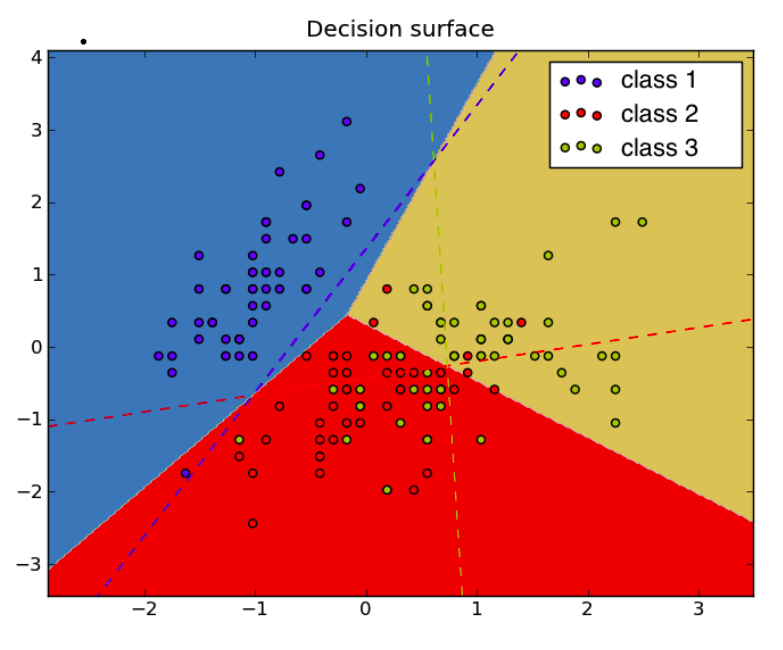
\includegraphics[scale=0.4]{multiclass.png}
    \caption{División del espacio para el clasificador discriminante con $k=3$. La línea punteada azul es $y_{1}$, la línea punteda roja es $y_{2}$ y la línea punteada amarilla es $y_{3}$}.
\end{figure}


\newpage
\noindent\textbf{P2. Detección de barcos en imágenes satelitales} (4 ptos) \href{https://nbviewer.jupyter.org/github/dgarridoa/T3ML/blob/master/solucion.ipynb}{\textcolor{blue}{\textbf{Código}}}
\vspace{5mm}

 El objetivo de esta pregunta es ayudar a abordar la difícil tarea de detectar la ubicación de grandes barcos usando imágenes satelitales. La importancia de esta tarea es múltiple, en particular, la detección automática de barcos podría facilitar el monitoreo de los niveles de actividad del puerto y el análisis de la cadena de suministro. El dataset disponible consiste de imágenes satelitales de barcos recopiladas en las áreas de la bahía de San Francisco y la bahía de San Pedro de California.  Este incluye 4000 imágenes 80x80 RGB, con la etiqueta "ship" (1) y "no-ship" (0). Más detalles sobre cómo cargar los datos y como extraer vectores de características a partir de una imagen en el notebook \textbf{tutorial.ipynb}. \textbf{Observación:} en el informe solo debe responder las preguntas planteadas, no adjunte código y debe ser lo más breve posible en los puntos a) y c).
\begin{enumerate}

\item[a)](0.5 ptos.) Cargue los datos y extraiga los vectores de características (vea \textbf{tutorial.ipynb}), pues las siguientes partes de esta pregunta serán todas en base a las características, no a las  \emph{entradas crudas}. Divida los datos de forma aleatoria en conjuntos de entrenamiento (70\%), validación (15\%) y testeo (15\%). 

\textbf{Observación:} Le puede ser útil la función \textit{train\_test\_split} de \textit{sklearn}.

\textbf{Solución}\\

Al particionar los datos en conjunto de entrenamiento, validación y testeo debemos asegurarnos que la distribución de los datos sea similar en ambos conjuntos, puesto, sino el modelo no podrá generalizar correctamente a observaciones que provienen de una distribución completamente distinta a la que generó los datos de entrenamiento. Una forma sencilla de hacer esto es seguir los siguientes pasos:

\begin{itemize}
    \item Barajar los datos, los datos pudieron ser recolectados siguiendo un patrón, por lo la distribución de las primeras 100 observaciones puede ser completamente diferente a las siguientes 100 observaciones, de hecho, en la tarea las primeras imágenes son de barcos y luego le siguen las que no tienen barcos (\textbf{0.2}).
    \item Una vez barajados los datos hacer muestro aleatorio independiente, esto garatizará que la distribución de los tres conjuntos sea más o menos similiar (\textbf{0.2}).
    \item Para garantizar reproducibilidad de los resultados es necesario fijar una semilla aleatoria (\textbf{0.1 ptos}).
\end{itemize}

\item[b)] (1.5 ptos.) Implemente la regresión logística bajo el método del descenso del gradiente estocástico (ver sección 4.5.2 del apunte). Su implementación debe incluir dos hiperparámetros:  la tasa de aprendizaje $\eta$, y el número de épocas de entrenamiento $e$, donde una época corresponde a una pasada por todo el conjunto de entrenamiento (pues recuerde que el gradiente estocástico solo usa una observación a la vez).  \\
Grafique la log-verosimilitud normalizada por el número de observaciones (eje y) versus el número de épocas (eje x), tanto para el conjunto de entrenamiento como el de validación para distintas tasas de aprendizaje, para ello considere $\eta \in  \{0.01, 0.05, 0.1\}$ y {épocas} $e\in \{1,\ldots, 100\}$. Luego, en base a los gráficos responda la siguiente pregunta:
¿Cuál es la configuración óptima de $\eta$ y \textit{épocas}? \textbf{Justifique su elección y explique qué pasa con tazas de aprendizaje muy grandes o pequeñas}.\\
\textbf{Observaciones:} La clase anterior debe ser escrita usando el stack de Python y Numpy, no está permitido el uso de algún solver para optimizar la log-verosimilitud. El archivo \textbf{tutorial.ipynb} cuenta con una plantilla a modo de guía para su implementación.

\textbf{Solución}\\

La probabilidad de "ship" viene dada por $P(y_{i}=1) = \frac{1}{1+e^{-w^{T}x_{i}}}=\sigma_{i}$ y la probabilidad de "no-ship" viene dada por $P(y_{i}=0) = 1-P(y_{i}=1)$ (puede ser al revés, depende de como se halla modelado) (\textbf{0.5 ptos fit}). Luego la asignación binaria del método \textit{predict} asigna a la clase "ship" si $P(y_{i}=1)\geq 0.5$ y a la clase "no-ship" si no (\textbf{0.1 ptos predict}). La log-verosimilitud (\textbf{0.2 ptos log\_verosimilitud}):
\begin{align*}
    l(w) = \sum_{i=1}^{N}y_{i}log(\sigma_{i})+(1-y_{i})log(1-\sigma_{i})
\end{align*}

\begin{figure}[H]
    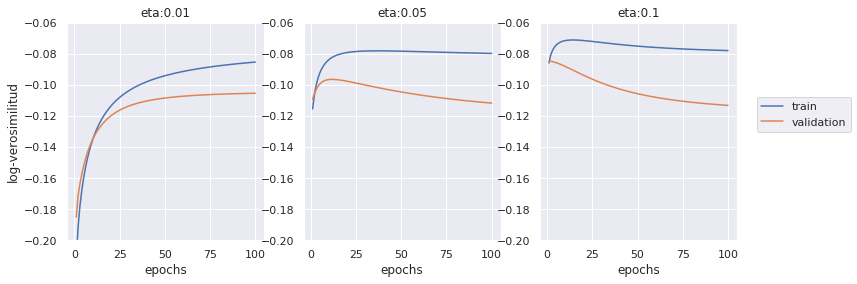
\includegraphics[scale=0.62]{log_likelihood.png}
    \caption{log-verosimilitud de la regresión logística tanto en el conjunto de entrenamiento como en el conjunto de test bajo el algoritmo de gradiente estocástico.}
\end{figure}

El objetivo es encontrar la combinación de hiperparámetros con mejor desempeño en el conjunto de validación, es decir, con mayor log-likelihood, en este caso particular fue ($\eta$, \textit{epochs}) = (0.1, 2) (\textbf{0.2 ptos}). En la Figura x se puede observar que para $\eta \in {0.05, 0.1}$ la log-likelihood alcanza un máximo en el conjunto de validación, tras este máximo a más épocas de entrenamiento el desempeño en validación comienza a empeorar y el de entrenamiento tiende a mejorar, observandosé un claro overfitting (\textbf{0.2 ptos}). El efecto de $\eta$ en el entrenamiento es la velocidad de convergencia, en este caso a mayor $\eta$ más rápidamente alcanza un máximo, en el caso de $\eta = 0.01$ que es el valor más pequeño para las 100 épocas aún no alcanza un máximo, por lo que podría seguir mejorando si aumentamos la cantidad de épocas de entrenamiento. Pequeñas tasas de aprendizaje requieren más épocas de entrenamiento dado que los pesos de una época a otra cambian ligeramente, en cambio tasas grandes de aprendizaje causan que el modelo converga demasiado rápido a soluciones subóptimas, como en el caso de $\eta=0.1$ donde se alcanza un máximo en entrenamiento y luego la log-likelihood empieza a empeorar (\textbf{0.3 ptos}). En la práctica se usan métodos de gradiente estocástico que adaptan la tasa de aprendizaje, donde la tasa de aprendizaje decrece en el número de épocas o batchs.

\item [c)] (1.0) Implemente el discriminante lineal de Fisher. En la sección 4.3 del apunte se describe cómo obtener $a$, con lo que luego podemos definir un umbral $b$ para asignar un $x$ a $\mathcal{C}_{1}$ si $a^{T}x\geq-b$ y a $\mathcal{C}_{2}$ en caso contrario. Para efectos de esta pregunta considere:
\begin{equation*}
    -b=a^{\top}\frac{1}{2}(\mu_{1}+\mu_{2})=\frac{1}{2}(m_{1}+m_{2})
\end{equation*}.\\ 
\textbf{Observaciones:} La clase anterior debe ser escrita usando el stack de Python y Numpy. El archivo \textbf{tutorial.ipynb} cuenta con una plantilla a modo de guía para su implementación. 

\textbf{Solución}\\
La asginación de una observación a la clase "ship" (1) si $a^{T}x\geq -b$ y la clase "no-ship" (2) si no, con $a=S_{W}^{-1}(\mu_{1}-\mu_{2})$, con $S_W =\sum_{n\in \mathcal{C}_{1}}(x_{n}-\mu_{1})(x_{n}-\mu_{1})^{T}+\sum_{n\in \mathcal{C}_{2}}(x_{n}-\mu_{2})(x_{n}-\mu_{2})^{T}$. Distribución del puntaje: \textbf{0.8 ptos fit} y \textbf{0.2 ptos predict}.

\item[d)] (1.0 pts.) ¿Cuál modelo (regresión logística o  discriminante de Fisher) tiene mejor desempeño en el conjunto de testeo? Para responder esta pregunta proponga y justifique una métrica para evaluar el desempeño de un método general de clasificación, luego, evalúe ambos clasificadores usados y compárelos. ¿Por qué cree usted que es necesario comparar ambos modelos en el conjunto de testeo en vez de el conjunto de entrenamiento o validación?
\\\textbf{Observaciones:} para el caso de la regresión logística considere la mejor configuración del punto b) y a la hora de escoger la métrica tenga en cuenta que las clases están \textbf{desbalanceadas}, i.e., la cantidad de elementos por clase es distinta.

\textbf{Solución}:

Justificación métrica (\textbf{0.5 ptos}). Debe proponerse una métrica adecuada para el dominio del problema que es discreto, si se proponen métricas para problemas de regresión dar 0 ptos. Además, la métrica debe permitir comparar ambos modelos, en este caso la verosimilitud no sería valida, dar 0 ptos en este caso. Si se proponen métricas que no consideran el desbalanceo de clases como accuracy dar la mitad del puntaje.\\ 

Una forma de minorizar el efecto de clases desbalanceadas es construir métricas que miden acertividad dándole más peso a la clase minoritaria que suele ser la clase que más nos interesa. En este caso la solución óptima es trabajar con matricez de utilidad, cuantificando el beneficio/costo de predecir bien/mal tanto la clase "ship" como "no-ship". En general, cuantificar esos costos y beneficios es una tarea difícil, por lo que alternativas más sencillas suelen trabajar con las tasas de acertividad (\textit{recall}) y precisión (\textit{precision}) de las clases y luego relizan promedios simples o harmónicos, por ejemplo, \textit{macro recall}, que es el promedio siemple entre la tasa de acertividad de todas las clases. En este caso el mejor modelo fue FLDA con un macro recall del 92.24\% por sobre la regresión logística que obtuvo un desempeño ligeramente inferior de un 90.96\%. 

El objetivo de toda tarea predictiva es desarrollar modelos con alta capacidad de generalización. Para medir esta capacidad hacemos una simulación, la cual consiste de seleccionar una muestra de nuestra datos, la cual asumimos que no sabemos su etiqueta y será el conjunto donde mediremos la verdadera capacidad predictiva de nuestros modelos de acuerdo a la métrica escogida. Este conjunto es distinto al de entrenamiento por que en este conjunto calibramos los parámetros de los modelos y al de validación ya que en este calibramos los hiperparámetros de uno de nuestros modelos. En el conjunto no debemos calibrar nada de nuestros modelos, ni siquera sus hiperparámetros, pues en una correcta simulación no deberíamos conocer de antemano la etiqueta, así de esta manera podemos medir la verdadera capacidad predictiva de los modelos (\textbf{0.5 ptos}).


\end{enumerate}

\noindent\textbf{P3. Proyecto curso} (1 pto)
\vspace{5mm}

Esta parte debe ser respondida por \textbf{un único} integrante del grupo, donde debe indicar los demás integrantes del grupo. Se habilitará una tarea aparte para su entrega en formato PDF cuya \textbf{extensión máxima es media página}.
\begin{itemize}
    \item[a)] (0.5 ptos) Enmarque su proyecto en algún tipo de aprendizaje (clasificación, regresión, clustering, aprendizaje, reforzado, etc.). Identifique según el caso el rol de sus variables, por ejemplo, si su proyecto es de clasificación, describa su variable independiente, sus características y sus clases. Si su proyecto no parece caber evidentemente en ninguno de estos casos, explíquelo en detalle y propongo cómo lo abordará desde el punto de Aprendizaje de Máquinas.
    \item[b)] (0.5 ptos) Proponga al menos 2 métodos para resolver su problema, fundamentando brevemente su elección.
\end{itemize}


\end{document}